\documentclass[a4paper,twocolumn,12pt]{article}
\usepackage[left=1.5cm, right=1.5cm, top=2cm,bottom=2cm]{geometry}
\usepackage{amsmath, amssymb, amsfonts}
\usepackage{enumerate}
\usepackage{tikz}
\begin{document} 
\section*{Piape Matemática} 
 
\subsection*{Módulo I}
\subsection*{Exercícios Aula 03}

\paragraph{1.} Classifique as afirmações em verdadeiras ou falsas:
\begin{enumerate}[a)]
\item Todo número natural também é inteiro. 
\item Todo número inteiro também é natural.  
\item Existem números inteiros que não são naturais.
\item Todo número racional é inteiro. 
\item Todo número inteiro é racional.
\item $\sqrt{2}$ é um número racional.
\item $\sqrt{2} \notin \mathbb{Q}$.
\item $\sqrt{2} \in \mathbb{R\backslash Q}$.
\end{enumerate}


\paragraph*{2. } As afirmações da questão 1 podem ser traduzidas em símbolos matemáticos. Associe os símbolos abaixo com as afirmações correspondentes:
\begin{enumerate}[a)]
  \item (\hspace{7mm}) $\sqrt{2} \in \mathbb{Q}$ 
  \item (\hspace{7mm}) $\mathbb{Z} \subseteq \mathbb{Q}$
  \item (\hspace{7mm}) $\mathbb{Q} \subseteq \mathbb{Z}$
  \item (\hspace{7mm}) $\mathbb{Z} \subseteq \mathbb{N}$
  \item (\hspace{7mm}) $\mathbb{N} \subseteq \mathbb{Z}$
\end{enumerate}

\paragraph*{3.} Dados os números abaixo, inclua eles no diagrama de Venn-Euler dos conjuntos numéricos:
\begin{minipage}{0.48\columnwidth}
  \begin{enumerate}[a)]
    \item $-3$
    \item $0$
    \item $1,\!89$
    \item $\frac{1}{2}$
    \item $\sqrt{2}$
  \end{enumerate}  
\end{minipage}
\begin{minipage}{0.48\columnwidth}
  \begin{enumerate}[a)]
    \setcounter{enumi}{5}
    \item $\pi$
    \item $\sqrt[3]{9}$
    \item $\frac{20}{4}$
    \item $\sqrt{-3}$
    \item $-\frac{5}{4}$
  \end{enumerate} 
\end{minipage}

{\centering 
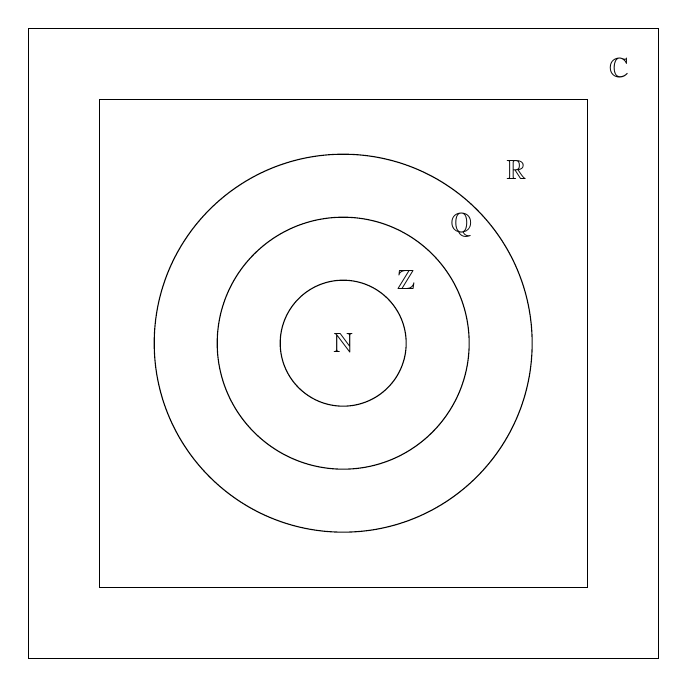
\begin{tikzpicture}
  \draw (-4,-4) rectangle (4,4);
  \draw (0,0) circle (0.8);
  \draw (0,0) circle (1.6);
  \draw (0,0) circle (2.4);
  \draw (-3.1,-3.1) rectangle (3.1,3.1);
  \node at (0,0) {$\mathbb{N}$};
  \node at (0.8,0.8) {$\mathbb{Z}$};
  \node at (1.5,1.5) {$\mathbb{Q}$};
  \node at (2.2,2.2) {$\mathbb{R}$};
  \node at (3.5,3.5) {$\mathbb{C}$};
\end{tikzpicture}
}

\vfill
% REMOVER OPERAÇÕES COM FRAÇÕES

{\footnotesize\color{darkgray}
\paragraph*{Gabarito} \hspace*{\fill}\\
\textbf{1.} a) Verdadeira; b) Falsa; c) Verdadeira; d) Falsa; e) Verdadeira; f) Falsa; g) Verdadeira; h) Verdadeira\\ 
\textbf{2.} a) f); b) e); c) b); d) c); e) d)\\
\textbf{3.}
\begin{flushright}
  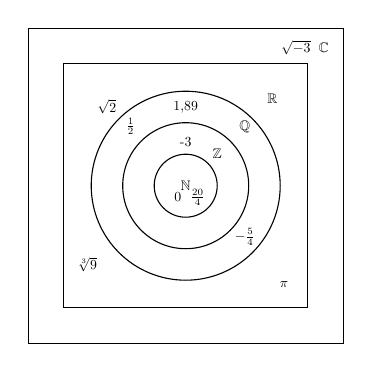
\begin{tikzpicture}[scale=0.5,every node/.style={scale=0.5}]
    \draw (-4,-4) rectangle (4,4);
    \draw (0,0) circle (0.8);
    \draw (0,0) circle (1.6);
    \draw (0,0) circle (2.4);
    \draw (-3.1,-3.1) rectangle (3.1,3.1);
    \node at (0,0) {$\mathbb{N}$};
    \node at (0.8,0.8) {$\mathbb{Z}$};
    \node at (1.5,1.5) {$\mathbb{Q}$};
    \node at (2.2,2.2) {$\mathbb{R}$};
    \node at (3.5,3.5) {$\mathbb{C}$};
    \node at (0,1.1){-3};
    \node at (-0.2,-0.3){0};
    \node at (0,2.0){1,89};
    \node at (-1.4,1.5){$\frac{1}{2}$};
    \node at (-2,2){$\sqrt{2}$};
    \node at (2.5,-2.5){$\pi$};
    \node at (-2.5,-2.0){$\sqrt[3]{9}$};
    \node at (0.3,-0.3){$\frac{20}{4}$};
    \node at (2.8, 3.5){$\sqrt{-3}$};
    \node at (1.5,-1.3){$-\frac{5}{4}$};
  \end{tikzpicture}
\end{flushright}
}
\end{document}